\documentclass[answers]{exam}

\usepackage[UTF8]{ctex}
\usepackage{fontspec}

\setCJKmainfont{SourceHanSerifCN-Regular}[
    Path = fonts/ ,
    Extension = .otf ,
    UprightFont = SourceHanSerifCN-Regular,
    BoldFont = SourceHanSerifCN-Bold,
]

\setCJKsansfont{SourceHanSansCN-Regular}[
    Path = fonts/ ,
    Extension = .otf ,
    UprightFont = SourceHanSansCN-Regular,
    BoldFont = SourceHanSansCN-Bold,
]

\usepackage{fullpage}
\usepackage{multicol}
\usepackage{color}
\usepackage{hyperref}
\usepackage{comment}

\usepackage{caption}
\usepackage{subcaption}

\usepackage{amsmath}
\usepackage{amssymb}
\usepackage{amsthm}
\usepackage{bm}
\usepackage{mathtools}

\newtheoremstyle{example}% name
{3pt}% Space above
{3pt}% Space below
{}% Body font
{}% Indent amount (empty = no indent, \parindent = para indent)
{\normalfont}% Thm head font
{}% Punctuation after thm head
{1em}% Space after thm head: " " = normal interword space;
% \newline = linebreak
{\textsf{\thmname{#1}\thmnumber{#2}\thmnote{#3}}}% Thm head spec (can be left empty, meaning `normal')

\theoremstyle{example}
\newtheorem{example}{例}

\renewenvironment{proof}{\noindent\textsf{证明}\quad}{\hfill $\square$\par}
\newtheorem{lemma}{引理}

\usepackage{algorithm}
\usepackage{algpseudocode}

\floatname{algorithm}{算法}
\renewcommand{\algorithmicrequire}{\textsf{输入:}}
\renewcommand{\algorithmicensure}{\textsf{输出:}}

\renewcommand{\solutiontitle}{}

\usepackage{tikz}
\usepackage{minted}


\title{算法与复杂性 \quad 作业十三}

\author{516021910528 - SHEN Jiamin}
\date{\today}

\begin{document}

\maketitle

\begin{questions}
    \section{0511}\label{sec:0511}

    \question 设计算法求出$n$个矩阵$M_1, M_2, \dots ,M_n$相乘最多需要多少次乘法,请给出详细的算法描述和时间复杂性

    \begin{solution}
        给定$n+1$个正整数$c_0,c_1, \dots , c_{n}$,
        其中$c_{i-1}$ 和 $c_{i}$ 为矩阵$M_i$的行数和列数,$1 \le i \le n$。

        记$M_{ij}$为$M_iM_{i+1} \dots M_j$的乘积,$Q(i,j)$为计算$M_{ij}$所需要的最多乘法数量,则
        \[
            Q(i,j) = \begin{cases}
                \max_{i \le k < j}{ \left\{ Q(i, k) + Q(k+1, j) + c_{i-1} c_k c_{j} \right\} } & , i < j \\
                0                                                                              & , i = j
            \end{cases}
        \]
        \textbf{伪代码见算法\ref{alg:0511:1}},算法的时间复杂度为$O(n^3)$。
    \end{solution}

    \begin{algorithm}[!ht]
        \caption{矩阵最多乘法次数}\label{alg:0511:1}
        \begin{algorithmic}[1]
            \Require {$n+1$个正整数$c[0 \dots n]$}
            \Ensure {最大乘法次数}
            \State $Q[1 \dots n][1 \dots n] \gets \left\{0\right\}$
            \For {$j \gets 2$ to $n$}
            \For {$i \gets j-1$ down to $1$}
            \State $precompute \gets c[i-1]c[j]$
            \For {$k \gets i$ to $j-1$}
            \State $t \gets Q[i][k] + Q[k+1][j] + c[k] \cdot precompute$
            \State $Q[i][j] \gets t$ if $Q[i][j] < t$
            \EndFor
            \EndFor
            \EndFor
            \State \Return $Q[1][n]$
        \end{algorithmic}
    \end{algorithm}

    \question 设有算法$A$能够在$O(i)$时间内计算一个$i$次多项式和一个$1$次多项式的乘积,
    算法$B$能够在$O(i \log i)$时间内计算两个$i$次多项式的乘积。
    现给定$d$个整数$n_1,n_2, \dots ,n_d$,设计算法求出满足$P(n_1)=P(n_2)= \dots =P(n_d)=0$
    且最高次项系数为$1$的$d$次多项式$P(x)$,并给出算法的时间复杂性。

    \begin{solution}
        满足$P(n_1)=P(n_2)= \cdots =P(n_d)=0$且最高次项系数为$1$的$d$次多项式$P(x)$为
        \[
            P(x) = (x-n_1)(x-n_2) \cdots (x-n_d)
        \]

        记$Q(i,j) = (x-n_i) \cdots (x-n_j)$,则$P(x) = Q(1,d)$
        \[
            Q(i,j) = \begin{cases}
                A(Q(i,j-1), (x-n_j))                 & , j-i+1 \equiv 1 \bmod 2 \\
                B(Q(i,(i+j-1)/2), Q((i+j-1)/2+1, j)) & , j-i+1 \equiv 0 \bmod 2
            \end{cases}
        \]

        \textbf{伪代码见算法\ref{alg:0511:2}}

        \newcommand{\pp}[1]{ \left( #1 \right) }
        \newcommand{\pb}[1]{ \left[ #1 \right] }
        \newcommand{\pT}[1]{ T\left( #1 \right) }
        \newcommand{\pO}[1]{ O\left( #1 \right) }

        设该算法运行所需时间为$T(d)$,则\[
            T(d) = \begin{cases}
                1                                                     & , d = 2              \\
                \pT{d-1} + \pO{d-1}                                   & , d \equiv 1 \bmod 2 \\
                2\pT{\frac{d}{2}} + \pO{\frac{d}{2} \log \frac{d}{2}} & , d \equiv 0 \bmod 2
            \end{cases}
        \]

        \begin{itemize}
            \item 当$d = 2^k$时,
                  \begin{align*}
                      \pT{2^k}
                      = & 2 \pT{ 2^{k-1} } + \pO{ (k-1)2^{k-1} }                         \\
                      = & 2^2 \pT{ 2^{k-2} } + \pO{ 2(k-2) 2^{k-2} +(k-1) 2^{k-1} }      \\
                      = & 2^2 \pT{ 2^{k-2} } + \pO{ \pb{ (k-2)+(k-1) } 2^{k-1} }         \\
                      = & 2^{k-1} \pT{2} + \pO{ \sum_{i=1}^{k-1} (k-i) 2^{k-1} }         \\
                      = & 2^{k-1} + \pO{ k^{2} 2^{k-1} } = \pO{ d \cdot \log^2 d }
                  \end{align*}
            \item 当$d = 2^k - 1$时,记$u_k = 2^k - 1$,且有$u_k - 1 = 2u_{k-1}$
                  \begin{align*}
                      \pT{2^k - 1} = \pT{u_k}
                      = & \pT{ u_k-1 } + \pO{ u_k-1 } = \pT{ 2 u_{k-1} } + \pO{ 2 u_{k-1} }                                                      \\
                      = & 2 \pT{ u_{k-1} } + \pO{ u_{k-1} \log\pp{ u_{k-1} } } + \pO{ 2 u_{k-1} }                                                \\
                      = & 2^2 \pT{ u_{k-2} } + \pO{ 2 u_{k-2} \log\pp{ u_{k-2} } + u_{k-1} \log\pp{ u_{k-1} } } + \pO{ 2^2 u_{k-2} + 2 u_{k-1} } \\
                      = & 2^{k-2} \pT{ u_{2} } + \pO{ \sum_{i=2}^{k-1} 2^{k-i-1}u_{i} \log\pp{ u_{i} } } + \pO{ \sum_{i=2}^{k-1} 2^{k-i} u_{i} } \\
                      = & \pO{ 3 \cdot 2^{k-2} } + \pO{ \sum_{i=2}^{k-1} 2^{k-i-1}\pp{2^i-1} i + \sum_{i=2}^{k-1} 2^{k-i} \pp{2^i-1} }           \\
                      %   = & 2^{k-2} \pT{ 3 } + \pO{ \sum_{i=2}^{k-1} 2^{k-i-1}\pp{2^i-1} \log\pp{ u_{i} } + \sum_{i=2}^{k-1} 2^{k-i} \pp{2^i-1} }                               \\
                      %   = & 2^{k-2} \pp{ \pT{ 2 } + \pO{ 2 } } + \pO{ \sum_{i=2}^{k-1} \pp{2^{k-1}-2^{k-i-1}} \log\pp{ u_{i} } + \sum_{i=2}^{k-1} \pp{2^{k}-2^{k-i}} }                 \\
                      %   = & \pO{ 3 \cdot 2^{k-2} } + \pO{ (k-2) 2^k + \sum_{i=2}^{k-1} 2^{k-1}\log\pp{ u_{i} } - \sum_{i=2}^{k-1} 2^{k-i-1}\log\pp{ u_{i} } - \sum_{i=1}^{k-2} 2^i } \\
                      %   = & \pO{ 2^{k-2} + (k-2) 2^k + 2 } + \pO{ \sum_{i=2}^{k-1} i \cdot 2^{k-1} - \sum_{i=2}^{k-1} i \cdot 2^{k-i-1} } \\
                      %   = & \pO{ 2^{k-2} + (k-2) 2^k + 2 } + \pO{ \pb{ 2^{k-2}\left(k^{2}-k-2\right) } - \pb{ -k+3 \times 2^{k-2}-1 } } \\
                      = & \pO{ 2^{k-2} k^{2}+3 \times 2^{k-2} k+k-3 \times 2^{k}+3 } = \pO{ 2^k k^2 } = \pO{ d \log^2 d }
                  \end{align*}
        \end{itemize}
    \end{solution}

    \begin{algorithm}[!ht]
        \caption{零点多项式}\label{alg:0511:2}
        \begin{algorithmic}[1]
            \Require {$d$个整数$n[1 \dots d]$}
            \Ensure {多项式}

            \Procedure{Q}{$n[1 \dots d]$}
            \If{ $d = 1$ }
            \State \Return $(-n[d], 1)$ \Comment{$x-n_d$}
            \ElsIf{ $d \equiv 0 \bmod 2$ }
            \State $P_1 \gets \Call{Q}{n[1 \dots d/2]}$
            \State $P_2 \gets \Call{Q}{n[d/2 + 1 \dots d]}$
            \State \Return $\Call{GivenAlgoB}{P_1,P_2}$
            \Else
            \State $P_1 \gets \Call{Q}{n[1 \dots d-1]}$
            \State $P_2 \gets \Call{Q}{n[d \dots d]}$
            \State \Return $\Call{GivenAlgoA}{P_1,P_2}$
            \EndIf
            \EndProcedure

            \State \Return $\Call{Q}{n}$
        \end{algorithmic}
    \end{algorithm}

    \question 将正整数$n$表示成一系列正整数之和:$n=n_1+n_2+ \dots +n_k$,
    其中$n_1 \ge n_2 \ge \dots \ge n_k \ge 1$,$k \ge 1$。
    正整数$n$的这种表示称为正整数$n$的划分,例如正整数6有如下11种不同的划分:
    \begin{center}
        \begin{tabular}{ccc}
            $ 6 $           &             &               \\
            $ 5+1 $         &             &               \\
            $ 4+2 $         & $ 4+1+1 $   &               \\
            $ 3+3 $         & $ 3+2+1 $   & $ 3+1+1+1 $   \\
            $ 2+2+2 $       & $ 2+2+1+1 $ & $ 2+1+1+1+1 $ \\
            $ 1+1+1+1+1+1 $ &             &               \\
        \end{tabular}
    \end{center}
    设计算法求正整数$n$的不同划分个数并证明其时间复杂性为$\Theta(n^2)$。

    \begin{solution}
        记$Q(n, m)$为最大数为$m$的$n$的所有划分,
        即$m = n_1 \ge n_2 \ge \dots \ge n_k \ge 1$。
        当一个划分中最大的数为$k$时,划分中剩余的部分为$Q(n-k,k)$,
        使用动态规划求解。
        \[
            P(n) = \bigcup_{1 \le m \le n} Q(n, m)
        \]其中
        \[
            Q(n, m) = \begin{cases}
                \bigcup_{1 \le k \le m, k<n} {\left\{ k \right\} \times Q(n-k, k) } & n > m \ge 1 \\
                \left\{ \left\{ n \right\} \right\}                                 & n = m       \\
            \end{cases}
        \]

        \textbf{代码见算法\ref{alg:0511:3}}

        求解$P(n)$,需要求解$\frac{n(n-1)}{2}$个子问题$Q$,所以时间复杂度为$\Theta(n^2)$
    \end{solution}

    \begin{algorithm}[!ht]
        \caption{正整数分划}\label{alg:0511:3}
        \inputminted{python}{alg-0511-03.py}
    \end{algorithm}


    \newpage %%%%%%%%%%%%%%%%%%%%%%%%%%%%%%%%%%%%%%%%%%%%%%%%%%%%%%%%%%%%%%%%%%%%%%%
    \section{0514}\label{sec:0514}

    \question 输入是由数轴上的区间所组成的集合,这些区间由它们的两个端点表示。
    设计$O(n \log n)$算法识别所有包含在集合中其它某个区间的区间。
    这个问题与二维平面极大点问题有什么关系

    例如输入:$(1,3), (2,8), (4,6), (5,7), (7,9)$,则输出为$(4,6)$和$(5,7)$

    \begin{solution}


        \textsf{极大点的定义} \quad
        {
            \kaishu
            设$p_1=(x_1,y_1)$和$p_2=(x_2,y_2)$是平面上的两个点,
            如果$x_1 \le x_2$并且$y_1 \le y_2$,则称$p_2$支配$p_1$,记为$p_1 \prec p_2$。
            点集$S$中的点$p$为极大点,意味着在$S$中找不到一个点$q$,$q \ne p$并且$p \prec q$,
            即$p$不被$S$中其它点支配。
        }

        区间$(x_1, y_1)$包含区间$(x_2, y_2)$当且仅当\[
            x_1 \le x_2 \wedge y_1 \ge y_2
        \]

        将区间用平面上的点表示,所有的点都在直线$y=x$上方。

        \begin{figure}[H]
            \centering
            \begin{subfigure}[b]{0.45\textwidth}
                \centering
                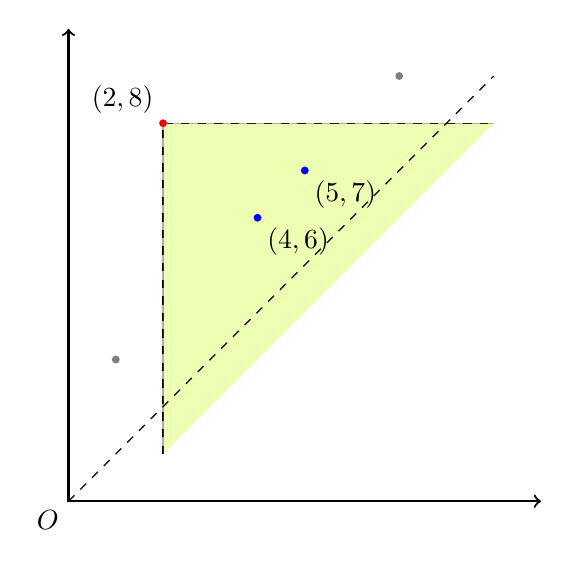
\begin{tikzpicture}[scale=0.6]
                    \coordinate (p1) at (1,3);
                    \coordinate (p2) at (2,8);
                    \coordinate (p3) at (4,6);
                    \coordinate (p4) at (5,7);
                    \coordinate (p5) at (7,9);

                    \draw[dashed] (2,1) -- (2,8) -- (9,8);
                    \draw[fill=lime, opacity=0.3] (2,1) -- (2,8) -- (9,8);

                    \filldraw [gray] (p1) circle (2pt);
                    \filldraw [red ] (p2) circle (2pt);
                    \filldraw [blue] (p3) circle (2pt);
                    \filldraw [blue] (p4) circle (2pt);
                    \filldraw [gray] (p5) circle (2pt);

                    \node [above left ] at (p2) {$(2,8)$};
                    \node [below right] at (p3) {$(4,6)$};
                    \node [below right] at (p4) {$(5,7)$};
                    \node [below left] at (0,0) {$O$};

                    \draw[thick, <->] (0,10) -- (0,0) -- (10,00);
                    \draw[dashed] (0,0) -- (9,9);
                \end{tikzpicture}
                \caption{$(x,y) \longmapsto (x,y)$}
            \end{subfigure}
            \begin{subfigure}[b]{0.45\textwidth}
                \centering
                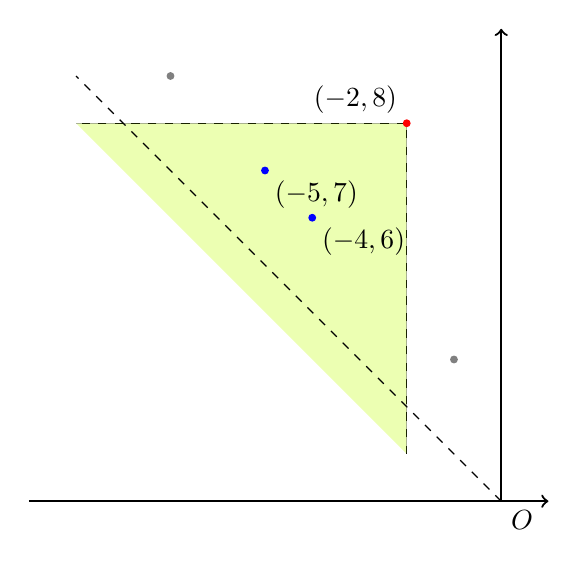
\begin{tikzpicture}[scale=0.6]
                    \coordinate (p1) at (-1,3);
                    \coordinate (p2) at (-2,8);
                    \coordinate (p3) at (-4,6);
                    \coordinate (p4) at (-5,7);
                    \coordinate (p5) at (-7,9);

                    \draw[dashed] (-2,1) -- (-2,8) -- (-9,8);
                    \draw[fill=lime, opacity=0.3] (-2,1) -- (-2,8) -- (-9,8);

                    \filldraw [gray] (p1) circle (2pt);
                    \filldraw [red ] (p2) circle (2pt);
                    \filldraw [blue] (p3) circle (2pt);
                    \filldraw [blue] (p4) circle (2pt);
                    \filldraw [gray] (p5) circle (2pt);

                    \node [above left ] at (p2) {$(-2,8)$};
                    \node [below right] at (p3) {$(-4,6)$};
                    \node [below right] at (p4) {$(-5,7)$};
                    \node [below right] at (0,0) {$O$};

                    \draw[thick, ->] (0,0) -- (0,10);
                    \draw[thick, ->] (-10,0) -- (1,0);
                    \draw[dashed] (0,0) -- (-9,9);
                \end{tikzpicture}
                \caption{$(x,y) \longmapsto (-x,y)$}
            \end{subfigure}
            \caption{将区间映射到二维平面上的点}
        \end{figure}

        为了与二维平面上极大点的定义相匹配,定义区间$(x,y)$映射到平面上的一点$(-x,y)$。
        则上述区间包含的等价条件相应地变为
        \[
            (x_2, y_2) \subseteq (x_1, y_1)
            \Longleftrightarrow -x_2 \le -x_1  \wedge y_2 \le y_1
            \Longleftrightarrow (-x_2, y_2) \prec (-x_1, y_1)
        \]

        所以该问题等价于在平面点集中,找出被其他任何一个点支配的所有点。
        即将区间集合映射到二维平面上的点集之后,找出二维平面中所有极大点的补集即可。

    \end{solution}

    \question  证明Graham算法是求凸包问题的一种最优算法

    \begin{solution}
        在$n$个点中选取$k$个点按一定顺序构成凸包,可能有$P(n, k)$种结果。
        由于$k$是未知的,所以共有\[
            \sum_{k = 3}^{n} P(n,k)
        \]种可能性。
        任取其中一种,选中正确的凸包的概率为\[
            p = \frac{1}{\sum_{k = 3}^{n} P(n,k)}
        \]
        其信息量为
        \begin{align*}
            I = & - \log p = \log \left( \sum_{k = 3}^{n} P(n,k) \right)
            = \log \left( \sum_{k = 3}^{n} \frac{n!}{(n-k)!} \right)
            =  \log \left( n! \sum_{k = 3}^{n} \frac{1}{(n-k)!} \right)          \\
            =   & \log n! + \log \left(\sum_{k = 3}^{n} \frac{1}{(n-k)!} \right)
            =  O(n \log n)
        \end{align*}

        一次比较操作能提供的信息量为$\log 2$,所以凸包问题的信息论下界为$O(n \log n)$。

        Graham算法的时间复杂度为$O(n\log n)$,与信息论下界同阶,是最优算法。

    \end{solution}

    \question 证明如果存在时间复杂度为$O(T(n))$的两个$n \times n$下三角矩阵的乘法,
    则存在时间复杂度为$O(T(n)+n^2)$的任意两个$n \times n$矩阵相乘的算法。

    \begin{solution}
        令$E$为$n$阶单位阵。设$A,B,C$均为$n$阶方阵,且$C = AB$。
        则矩阵\[
            Q = \begin{pmatrix}
                E & O & O & O \\
                B & E & O & O \\
                O & A & E & O \\
                O & O & B & E
            \end{pmatrix}
        \]是$4n$阶的下三角方阵。则有
        \[
            Q^2 = \begin{pmatrix}
                E  & O  & O  & O \\
                2B & E  & O  & O \\
                AB & 2A & E  & O \\
                O  & BA & 2B & E
            \end{pmatrix}
        \]

        构造矩阵$Q$需要时间$(4n)^2$,作矩阵乘法需要时间$T(4n)$,取出$AB$的值需要时间$n^2$。

        因此该算法的时间复杂度为$O(T(4n) + 17n^2)$。
        在假设$T(cn) = T(n)$的条件下,该复杂度即为$O(T(n)+n^2)$。
    \end{solution}

    \question  如果在序列$x_1,x_2, \dots ,x_n$中,存在某个$i$使$x_i$是序列中的最小者,
    且序列\[ x_i,x_{i+1}, \dots ,x_n,x_1,\dots, x_{i-1} \]是递增的,
    则称序列$x_1,x_2, \dots ,x_n$是循环序列。
    设计算法找出循环序列中最小元素的位置。
    为简单起见,假设该位置是唯一的。
    证明你的算法是最优的。

    \begin{solution}
        遍历整个序列以寻找最小值的时间复杂度为$O(n)$。

        在$n$个数组中随机选取一个数,该数是序列中最小的值的概率为$p = 1 / n$,信息量为$\log n$。
        下面给出一种时间复杂度为$O(\log n)$的算法,该算法的时间复杂度达到了问题的信息论下界,是一个最优算法。

        若序列$\left\{x_i\right\}$是递增的,则$\forall i,j : i < j \rightarrow x_i < x_j$。
        所以,若$\exists i < j : x_i > x_j $,则该序列是非增的;
        又因为该序列是循环递增的,所以序列的极值点一定在$i,j$之间。

        \textbf{伪代码见算法\ref{alg:0514:4}}

        该算法类似于二分查找,每次搜索范围减半直到找到最小值,其时间复杂度为$O(\log n)$。

    \end{solution}

    \begin{algorithm}[!ht]
        \caption{循环递增序列的极值点}\label{alg:0514:4}
        \begin{algorithmic}[1]
            \Require {序列$x[1 \dots n]$}
            \Ensure {$\mathrm{argmin}_i x_i$}
            \State $left \gets 1, right \gets n$
            \If { $x[left] < x[right]$ }    \Comment{序列是有序的}
            \State \Return $left$
            \Else
            \Repeat
            \State $mid \gets \frac{left + right}{2}$
            \If { $x[mid] < x[right]$ }     \Comment{$(mid, right)$是有序的}
            \State $right \gets mid$
            \Else                           \Comment{$(left, mid)$是有序的}
            \State $left \gets mid$
            \EndIf
            \Until{$right - left \le 1$}
            \State \Return $right$
            \EndIf
        \end{algorithmic}
    \end{algorithm}

\end{questions}

\end{document}